%%%%%%%%%%%%%%%%%%%%%%%%%%%%%%%%%%%%%%%%%%%%%%%%%%%%%%%%%%%%%%%%%%%%%%%%%%%%%%%%
%%%%%%%%%%%%%%%%%%%%%%%%% TOGGLES, CONSTANTS, SETTINGS %%%%%%%%%%%%%%%%%%%%%%%%%
%%%%%%%%%%%%%%%%%%%%%%%%%%%%%%%%%%%%%%%%%%%%%%%%%%%%%%%%%%%%%%%%%%%%%%%%%%%%%%%%

\newcount\Chatty  % whether to show our notes-to-selves in the pdf
\newcount\Drafty  % whether to show a timestamp in the pdf
\Chatty  = 1 % 0 for final copy; 1 for draft
\Drafty  = 0 % 0 for final copy; 1 for draft

%%%%%%%%%%%%%%%%%%%%%%%%%%%%%%%%%%%%%%%%%%%%%%%%%%%%%%%%%%%%%%%%%%%%%%%%%%%%%%%%
%%%%%%%%%%%%%%%%%%%%%%%%% DOCUMENT CLASS AND PACKAGES %%%%%%%%%%%%%%%%%%%%%%%%%%
%%%%%%%%%%%%%%%%%%%%%%%%%%%%%%%%%%%%%%%%%%%%%%%%%%%%%%%%%%%%%%%%%%%%%%%%%%%%%%%%

\documentclass[article,twocolumn]{memoir}
%\usepackage[utf8]{inputenc} % apparently not needed
\usepackage{amsmath}
\usepackage{amssymb}
\usepackage{amsthm}
\usepackage[calc, useregional, showseconds=false, showzone=false]{datetime2}
% also needs a line like the following in the file latexmkrc:
% $ENV{'TZ'}='America/New_York';
% ugh, except GitHub Actions won't respect that so instead we're setting the
% timezone to UTC and then doing black magic here in the latex source to compute
% the timezone.
\usepackage{xcolor} % used in chatty macros
\usepackage{tikz}
\usepackage{graphicx}
\usepackage{hyperref}
\hypersetup{colorlinks=true,urlcolor=blue}
\usepackage{emoji}

%%%%%%%%%%%%%%%%%%%%%%%%%%%%%%%%%%%%%%%%%%%%%%%%%%%%%%%%%%%%%%%%%%%%%%%%%%%%%%%%
%%%%%%%%%%%%%%%%%%%%%%%%%%%%% COMMANDS AND MACROS %%%%%%%%%%%%%%%%%%%%%%%%%%%%%%
%%%%%%%%%%%%%%%%%%%%%%%%%%%%%%%%%%%%%%%%%%%%%%%%%%%%%%%%%%%%%%%%%%%%%%%%%%%%%%%%

\newcommand{\dreev} [1]{\ifnum\Chatty=1 \textcolor{purple}{dreev:  [#1]} \fi}
\newcommand{\alice} [1]{\ifnum\Chatty=1 \textcolor{red}   {alice:  [#1]} \fi}
\newcommand{\bob}   [1]{\ifnum\Chatty=1 \textcolor{blue}  {bob:    [#1]} \fi}
\newcommand{\carol} [1]{\ifnum\Chatty=1 \textcolor{orange}{carol:  [#1]} \fi}
\newcommand{\daphne}[1]{\ifnum\Chatty=1 \textcolor{teal}  {daphne: [#1]} \fi}

% Utter black magic for doing timezone conversion for the draft timestamp...
% Via https://tex.stackexchange.com/questions/634804/how-to-change-the-timezone
\newcommand{\datetimemagic}[2]{\DTMsavenow{now}\DTMtozulu{now}{cz}
  \DTMsaveaszulutime{cx}{\DTMfetchyear{cz}}{\DTMfetchmonth{cz}}
  {\DTMfetchday{cz}}{\DTMfetchhour{cz}}{\DTMfetchminute{cz}}
  {\DTMfetchsecond{cz}}{#2}{00}\DTMdisplay{\DTMfetchyear{cx}}
  {\DTMfetchmonth{cx}}{\DTMfetchday{cx}}{}{\DTMfetchhour{cx}}
  {\DTMfetchminute{cx}}{\DTMfetchsecond{cx}}{#1}{00}}
% And here's even more unDRY ugliness because I don't know what I'm doing...
\newcommand{\datemagic}[2]{\DTMsavenow{now}\DTMtozulu{now}{cz}
  \DTMsaveaszulutime{cx}{\DTMfetchyear{cz}}{\DTMfetchmonth{cz}}
  {\DTMfetchday{cz}}{\DTMfetchhour{cz}}{\DTMfetchminute{cz}}
  {\DTMfetchsecond{cz}}{#2}{00}\DTMdisplaydate{\DTMfetchyear{cx}}
  {\DTMfetchmonth{cx}}{\DTMfetchday{cx}}{}}

% Set this to, eg, -08/+08 for Pacific Time in winter, -07/+07 in summer. Woof.
\newcommand{\tstamp}{\ifnum\Drafty=1 
  \textcolor{red}{DRAFT~\datetimemagic{-07}{+07}} \else 
  \datemagic{-07}{+07}
\fi}

\hfuzz=2pt % Don't bother to report overfull hboxes if over-edge is < 2pt
\vfuzz=2pt % Same for overfull vboxes (maybe just works for hfuzz?)

%\newcommand{\BibTeX}{\rm B\kern-.05em{\sc i\kern-.025em b}\kern-.08em\TeX}

%%%%%%%%%%%%%%%%%%%%%%%%%%%%%%%%%%%%%%%%%%%%%%%%%%%%%%%%%%%%%%%%%%%%%%%%%%%%%%%%
%%%%%%%%%%%%%%%%%%%%%% TITLE, AUTHORS, ABSTRACT, KEYWORDS %%%%%%%%%%%%%%%%%%%%%%
%%%%%%%%%%%%%%%%%%%%%%%%%%%%%%%%%%%%%%%%%%%%%%%%%%%%%%%%%%%%%%%%%%%%%%%%%%%%%%%%

\newcommand{\longtitle}{The Snake Eyes Paradox}
%\newcommand{\shorttitle}{Snake Eyes} % for page headers

\title{\HUGE\textbf{\longtitle}}
\author{Daniel M. Reeves\\dreev@beeminder.com}
%\affiliation{\institution{Beeminder}}
\date{\protect\tstamp} % need protection from black magic, apparently

%\begin{abstract}
%The answer is 1/36.
%\end{abstract}

%\keywords{Probability, Math puzzles}

%%%%%%%%%%%%%%%%%%%%%%%%%%%%%%%%%%%%%%%%%%%%%%%%%%%%%%%%%%%%%%%%%%%%%%%%%%%%%%%%
%%%%%%%%%%%%%%%%% START DOCUMENT, SET UP HEADERS, DO MAKETITLE %%%%%%%%%%%%%%%%%
%%%%%%%%%%%%%%%%%%%%%%%%%%%%%%%%%%%%%%%%%%%%%%%%%%%%%%%%%%%%%%%%%%%%%%%%%%%%%%%%

\begin{document}
\pagestyle{headings}
\maketitle

%%%%%%%%%%%%%%%%%%%%%%%%%%%%%%%%%%%%%%%%%%%%%%%%%%%%%%%%%%%%%%%%%%%%%%%%%%%%%%%%
%%%%%%%%%%%%%%%%%%%%%%%%%%%%%%%% MAIN DOCUMENT %%%%%%%%%%%%%%%%%%%%%%%%%%%%%%%%%
%%%%%%%%%%%%%%%%%%%%%%%%%%%%%%%%%%%%%%%%%%%%%%%%%%%%%%%%%%%%%%%%%%%%%%%%%%%%%%%%

\chapter*{Problem Statement}

You are offered a gamble.
A pair of six-sided dice are rolled and unless they come up snake eyes you get a bajillion dollars. 
If they do come up snake eyes, you're devoured by snakes.

So far it sounds like you have a 1/36 chance of dying, right?

Now the twist. 
First, I gather up an unlimited number of people willing to play the game, including you. 
I take 1 person from that pool and let them play. 
Then I take 2 people and have them play together, where they share a dice roll and either get the bajillion dollars each or both get devoured. 
Then I do the same with 4 people, and then 8, 16, and so on.

At some point we expect one of those groups will be devoured by snakes---hopefully not the group you're in---and then I stop.
Is the probability that you'll die, given that you're chosen to play, still 1/36?

\vspace{1em}

\textbf{Argument for NO:}
Due to the doubling, the final group of people that die is slightly bigger than all the surviving groups put together. 
So if you're chosen to play you have about a 50\% chance of dying!
\emoji{grimacing-face}
\emoji{snake}

\vspace{1em}

\textbf{Argument for YES:}
The dice rolls are independent and whenever you're chosen, what happened in earlier rounds is irrelevant.
Your chances of death are the chances of snake eyes on your round: 1/36.
\emoji{grinning-face-with-sweat}

\vspace{1em}

So which is it? 
What's your probability of dying, conditional on being chosen to play?

\newpage

Some clarifications:

\begin{enumerate}
\item The game is not adversarial and the dice rolls are independent and truly random.
\item Choosing each group also happens uniformly randomly and without replacement.
\item The question is about the unrealistic case of an unbounded number of people but we can cap it and say that if no one has died after $N$ rounds then the game ends and no one dies. 
We just need to then find the limit as $N$ goes to infinity. 
% SCHDEL in which case the probability that no one dies goes to zero.
\item Importantly, in the finite version it's possible for no one to die. 
The probability of that approaches zero as the size of the pool approaches infinity.
\end{enumerate}

\vspace{2em}
\noindent
\emph{Don't turn the page until you're ready for the solution!}

\vspace{2em}
\noindent
\emph{(Btw, this is only a veridical paradox. There's an unambiguously correct answer.)}

\newpage

\chapter*{Solution}

We want the probability that you die given that you're chosen to play, 
$\Pr(\text{death} \mid \text{chosen})$.
It seems like half the people who are chosen die, but let's Bayes it out carefully:

\begin{equation*}
\begin{split}
\Pr(\text{death} \mid \text{chosen}) & =
\frac{\Pr(\text{chosen} \mid \text{death}) \Pr(\text{death})}{\Pr(\text{chosen})} \\
& = \frac{1\cdot\Pr(\text{death})}{\Pr(\text{chosen})}.
\end{split}
\end{equation*}

In the uncapped case, that conditional probability is undefined. 
You're part of an infinite pool so you have a 0\% chance of being chosen and a 0\% chance of dying. 
The probability we want is 0/0. 
\emph{*robot-with-smoke-coming-out-of-its-ears-emoji*}

Since we can't directly calculate the probability in the infinite case, we have to take a limit.

\vspace{2em}

To get a feel for where we're going, suppose you're 1 person in a huge but finite pool.
Now suppose you're actually chosen. 
There are two ways that can happen: 
\begin{enumerate}
\item The pool runs out and everyone survives.
\item The pool doesn't run out and you have about a 50\% chance of dying. 
\end{enumerate}
But knowing that you're chosen is Bayesian evidence that we had many, many rounds of survival. 
If an early group died then most of the pool wasn't chosen, so probably you weren't chosen.

Thinking like a Bayesian means shifting your probability in light of evidence by seeing how surprised you'd be in various universes by that evidence.
If an early group died then most people aren't chosen and in that universe you're surprised to be chosen. 
If \emph{no} group died then everyone was chosen and in that universe you're fully unsurprised that you were chosen. 
That's the sense in which being chosen is Bayesian evidence that more people survived. 
In particular it's at least weak evidence that everyone survived.

So even with an absurdly huge pool of people, where there's \emph{essentially} a 0\% chance of everyone surviving, if you know you were chosen (which itself has near zero probability, but if) then that means you're more likely in that essentially-0\%-probability universe where everyone survives.

\vspace{2em}

Enough hand-waving and appeals to intuition.
Let's Bayes it out to see what 
$\Pr(\text{death} \mid \text{chosen})$
is exactly, in the version where we stop after $N$ rounds.
Once we have that, we can take the limit as $N$ goes to infinity.

First, let $M$ be the size of the pool:

$$M = \sum_{i=0}^{N-1} 2^i = 2^N-1.$$

And let $p$ be the probability of snake eyes, 1/36.
We can now compute the probability of being chosen by summing up 
(1) the probability you're chosen for the first round, $1/M$, plus 
(2) the probability that the first group survives, $1-p$, and that you're chosen for the 2nd round, $2/M$, plus 
(3) the probability that the first two groups survive and you're chosen for the 3rd round, etc.
Writing that out as an equation gives this:

\begin{align*}
\Pr(\text{chosen}) & = 
\begin{aligned}[t]
\tfrac{1}{M} & + (1-p)      \tfrac{2}{M} \\
             & + (1-p)^2    \tfrac{4}{M} \\
             & + (1-p)^3    \tfrac{8}{M} \\
             & + \ldots                  \\
             & + (1-p)^{N-1}\frac{2^{N-1}}{M}
\end{aligned} \\
& = \sum_{i=0}^{N-1} \tfrac{1}{M} 2^i(1-p)^i.
\end{align*}

For $\Pr(\text{death})$ the calculation is very similar but every term is multiplied by $p$.
To die, you have to be chosen and then roll snake eyes.
This can happen on any round, all of which are mutually exclusive.
We can then factor that $p$ out and we have

$$
\Pr(\text{death}) = p\cdot\Pr(\text{chosen}).
$$

Working out that expression for $\Pr(\text{chosen})$ wasn't even necessary!
We compute $\Pr(\text{death} \mid \text{chosen})$ like so:

\begin{equation*}
\begin{split}
\Pr(\text{death} \mid \text{chosen}) & = 
\frac{\Pr(\text{death})}{\Pr(\text{chosen})} \\
& = \frac{p\cdot\Pr(\text{chosen})}{\Pr(\text{chosen})} = 
p.
\end{split}
\end{equation*}

It doesn't depend on $N$ at all!
The limit as $N$ goes to infinity is just... 
$p$ or 1/36, the probability of rolling snake eyes.
\qedsymbol{}

\vspace{2em}
\noindent
\emph{Source: This is a variant of the Shooting-Room Paradox.
Googling that yields a sea of confusion and wrongness and paywalled philosophy papers so I wrote this.}

%%%%%%%%%%%%%%%%%%%%%%%%%%%%%%%%%%%%%%%%%%%%%%%%%%%%%%%%%%%%%%%%%%%%%%%%%%%%%%%%

\chapter*{Acknowledgments}

Thanks to 
Greta Goodwin, 
Bethany Soule, 
Christopher Moravec,
and Stan Wagon, as well as
CesiumLifeJacket and Nix and others in the PEAR Discord for helpful discussion.

Thanks also to Manifold Markets where I 
\href{https://manifold.markets/dreev/is-the-probability-of-dying-in-the}{posed this question}.
The market converged to the correct answer amidst heated discussion in the comments:

\vspace{2em}
\noindent
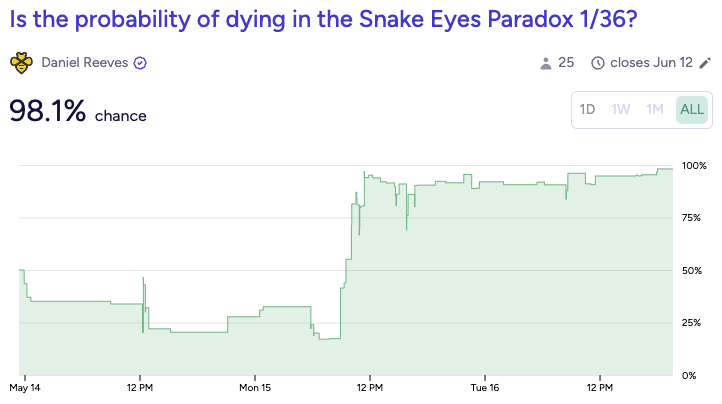
\includegraphics[width=\linewidth]{manifold-snakeeyes}


% random unrelated thing i wanted rendered:
%$$
%\mathop{\mathrm{arg\,max}}_{a \in \text{Actions}} \text{EU}(a)
%$$

\end{document}

%%%%%%%%%%%%%%%%%%%%%%%%%%%%%%%%%%%%%%%%%%%%%%%%%%%%%%%%%%%%%%%%%%%%%%%%%%%%%%%%
%%%%%%%%%%%%%%%%%%%%%%%%%%%%%%%% SCRATCH NOTES %%%%%%%%%%%%%%%%%%%%%%%%%%%%%%%%%
%%%%%%%%%%%%%%%%%%%%%%%%%%%%%%%%%%%%%%%%%%%%%%%%%%%%%%%%%%%%%%%%%%%%%%%%%%%%%%%%

To review, the uncapped version of the problem is not well posed because we have to condition on something (being chosen to play out of an infinite pool) that has probability zero.
Relatedly, the expected value of the number of people chosen to play is infinite, as is the expected number of deaths.
So we need to consider a finite version and take the limit.
But in the finite version there are two ways you can survive.
First, if the game ends in death and you're chosen to play then you have about a 50% chance.
Second, if the game ends by exhausting the pool, you definitely are chosen and definitely survive.
The probability of exhausting the pool is $(1-p)^N$ -- not rolling snake eyes $N$ times in a row.

The key intuition here is that, first, if there's a small pool of people then there's a good chance we exhaust the pool and everyone survives.
Second, if the pool is huge then probably you won't be chosen but \emph{if} you're chosen, that's Bayesian evidence that a lot of the pool got used up, which is Bayesian evidence that everyone survives.
The probability of both you being chosen and everyone surviving go to zero as the pool size grows, but the conditional probability stays fixed.
In the limit you have a 0\% chance of being chosen and
... I seem to be repeating myself here...

This really is quite subtle. 
I think that if we condition on some group dying then you do get an answer of 1/2. 
And in the unbounded case we know a group will eventually die. 
So how the heck does it change anything by conditioning on something that we know is definitely going to happen anyway?

And I think the answer is that it does matter. 
"No one ever dies" is one of the possible outcomes of an infinite sequence of dice rolls, even though it has probability zero.


https://link.springer.com/article/10.1023/A:1005100407551
